\documentclass[aspectratio=169, 10pt]{beamer}

\usepackage{bm} % bold math
\usepackage{fontspec}
\usepackage{minted}
\usepackage{pgf-pie}
\usepackage{tikz}
\usepackage{graphicx}
\newcommand\sbullet[1][.5]{\mathbin{\vcenter{\hbox{\scalebox{#1}{$\bullet$}}}}}

% Custom commands and environments
\makeatletter
\newcommand\version[1]{\renewcommand\@version{#1}}
\newcommand\@version{}
\def\insertversion{\@version}

\newcommand\course[1]{\renewcommand\@course{#1}}
\newcommand\@course{}
\def\insertcourse{\@course}

\newcommand\coursetitle[1]{\renewcommand\@coursetitle{#1}}
\newcommand\@coursetitle{}
\def\insertcoursetitle{\@coursetitle}

\newcommand\lecturenumber[1]{\renewcommand\@lecturenumber{#1}}
\newcommand\@lecturenumber{}
\def\insertlecturenumber{\@lecturenumber}
\makeatother

\newcommand{\slidetitle}[1]{{\xbseries \large \structure{#1}} \bigskip}
\newcommand{\term}[1]{{\color{blue} #1}}
\newcommand{\leftspace}{\hspace{1em}}
\newcommand{\inlinearrow}{
  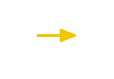
\begin{tikzpicture}[baseline]
    \node [anchor=base] (x) {};
    \draw [rawarrow] (x.mid west) -- ($(x.mid west) + (2em,0)$);
  \end{tikzpicture}
}

\newenvironment{slide}
{\begin{frame}[fragile,environment=slide]\vskip0pt plus 1filll}
{\vskip0pt plus 1filll\end{frame}}

% LaTeX

\setlength{\leftmargini}{1em}

% Common Information

\author{Talia Xu}
\course{COMPSCI 340}
\coursetitle{Operating Systems}
\date{2024 Semester 2}

% fontspec

\defaultfontfeatures{Ligatures=TeX}
% \setmainfont{Domine}
\setsansfont{Inter}[
  FontFace={ul}{n}{Font=*-Thin},
  FontFace={el}{n}{Font=*-ExtraLight},
  FontFace={l}{n}{Font=*-Light},
  FontFace={sb}{n}{Font=*-SemiBold},
  FontFace={eb}{n}{Font=*-ExtraBold},
  FontFace={xb}{n}{Font=*-Black},
]
\setmonofont[Contextuals=AlternateOff, Ligatures=TeXOff]{Iosevka}[
  FontFace={xb}{n}{Font=*-Heavy},
]

%% Font Weights

\DeclareRobustCommand{\ulseries}{\fontseries{ul}\selectfont}
\DeclareTextFontCommand{\textul}{\ulseries}
\DeclareRobustCommand{\elseries}{\fontseries{el}\selectfont}
\DeclareTextFontCommand{\textel}{\elseries}
\DeclareRobustCommand{\lseries}{\fontseries{l}\selectfont}
\DeclareTextFontCommand{\textl}{\lseries}
\DeclareRobustCommand{\sbseries}{\fontseries{sb}\selectfont}
\DeclareTextFontCommand{\textsb}{\sbseries}
\DeclareRobustCommand{\ebseries}{\fontseries{eb}\selectfont}
\DeclareTextFontCommand{\texteb}{\ebseries}
\DeclareRobustCommand{\xbseries}{\fontseries{xb}\selectfont}
\DeclareTextFontCommand{\textxb}{\xbseries}

% tikz

\usetikzlibrary{
  arrows,
  arrows.meta,
  automata,
  backgrounds,
  calc,
  decorations.pathreplacing,
  matrix,
  positioning,
  overlay-beamer-styles,
  shapes,
  shapes.multipart,
  tikzmark,
}

\tikzstyle{rawarrow} = [
  -{Latex[round]},
  line width=1pt,
  yellow,
  shorten >=3pt,
  shorten <=3pt,
  font=\small,
  text=black,
]

\tikzstyle{arrow} = [
  -{Latex[round]},
  line width=1pt,
  yellow,
  shorten >=3pt,
  shorten <=3pt,
  transform canvas={yshift=3pt},
  font=\small,
  text=black,
]

\newcommand{\tikzmarkcoord}[1]{([yshift=3pt]pic cs:#1)}

% minted

\setminted{style=eyolfson, fontsize=\small, escapeinside=||}
\setmintedinline{fontsize=\normalsize}

% hyperref

\hypersetup{colorlinks, urlcolor=blue}

% beamer
\setbeamersize{text margin left=16mm, text margin right=16mm}
\setbeamertemplate{itemize items}[circle]
\setbeamercolor{item}{fg=black}
\setbeamercolor{structure}{fg=darkblue}
\setbeamerfont{frametitle}{series=\bfseries, parent=structure}
\setbeamertemplate{navigation symbols}{}
\setbeamertemplate{headline}{}
\setbeamertemplate{footline}{
  \begin{tikzpicture}[
    remember picture,
    overlay,
    shift={(current page.south west)},
  ]
    \path [fill=gray] (144mm, 0) -- (160mm, 16mm) -- (160mm, 0);
    \node [inner sep=3.5mm, outer sep=0, text=black, anchor=base east,
           align=right, yshift=3.5mm]
          at (current page.south east) {\ttfamily \small \insertframenumber{}};
  \end{tikzpicture}
}
\setbeamertemplate{title page}{
  \begin{tikzpicture}[
    remember picture,
    overlay,
    shift={(current page.south west)},
    background rectangle/.style={fill=darkblue},
    show background rectangle,
  ]
    \node [anchor=center, align=center, text=white, text width=40mm, scale=3.2]
          at (\paperwidth / 2, \paperheight * 2 / 3)
          {\xbseries \inserttitle{}};
    \node [anchor=base west, align=left, inner sep=0, text=white, yshift=2.5mm]
          at (16mm, \paperheight / 3)
          {\insertdate{} \insertcourse{}: \insertcoursetitle{}};
    \node [anchor=base west, align=left, inner sep=0, text=white, yshift=-2.5mm]
          at (16mm, \paperheight / 3)
          {\insertauthor};
    \node [anchor=base east, align=right, inner sep=0, text=white, yshift=2.5mm]
          at (144mm, \paperheight / 3)
          {Lecture \insertlecturenumber{}};
    \node [anchor=base east, align=right, inner sep=0, text=white,
           yshift=-2.5mm]
          at (144mm, \paperheight / 3)
          {\ttfamily \insertversion{}};
    \node [align=center, anchor=south, inner sep=0, text=white, yshift=3.5mm]
          (license) at (\paperwidth / 2, 0)
          {\fontsize{7pt}{7pt}\selectfont This  work is licensed under a
           \href{http://creativecommons.org/licenses/by-sa/4.0/}
                {\color{lightblue} Creative Commons Attribution-ShareAlike 4.0
                 International License}};
  \end{tikzpicture}
}

% xcolor

%% Primary Colour

\definecolor{pantone655}{RGB}{0, 42, 92} % #002a5c
\colorlet{darkblue}{pantone655}

%% Secondary Colours

\definecolor{pantone633}{RGB}{0, 139, 176} % #008bb0
\colorlet{blue}{pantone633}

\definecolor{pantonewarmred}{RGB}{220, 70, 51} % #dc4633
\colorlet{red}{pantonewarmred}

\definecolor{pantone3285}{RGB}{0, 161, 137} % #00a189
\colorlet{cyan}{pantone3285}

\definecolor{pantone7722}{RGB}{13, 83, 77} % #0d534d
\colorlet{darkcyan}{pantone7722}

\definecolor{pantone376}{RGB}{141, 191, 46} % #8dbf2e
\colorlet{green}{pantone376}

\definecolor{pantone2613}{RGB}{109, 36, 122} % #6d247a
\colorlet{violet}{pantone2613}

\definecolor{pantone2985}{RGB}{111, 199, 234} % #6fc7ea
\colorlet{lightblue}{pantone2985}

\definecolor{pantone227}{RGB}{171, 19, 104} % #ab1368
\colorlet{magenta}{pantone227}

\definecolor{pantone7406}{RGB}{241, 197, 0} % #f1c500
\colorlet{yellow}{pantone7406}

%% Neutrals

\definecolor{pantonecoolgray2}{RGB}{208, 209, 201} % #d0d1c9
\colorlet{gray}{pantonecoolgray2}


\lecturenumber{19}
\title{Sockets}
\version{2.0.0}

\begin{document}
  \begin{frame}[plain, noframenumbering]
    \titlepage
  \end{frame}

  \begin{slide}
    
    \slidetitle{Sockets are Another Form of IPC}

    We've seen pipes and signals

    \leftspace{}We also talked about shared memory
    \medskip

    Previous IPC assume that the processes are on the same physical
    machine
    \bigskip

    Sockets enable IPC between physical machines, typically over the network

  \end{slide}

  \begin{slide}
    
    \slidetitle{Servers Follow 4 Steps to Use Sockets}

    These are all system calls, and have the usual C wrappers:

    \begin{enumerate}
      \item \texttt{socket}

        \leftspace{}Create the socket
      \item \texttt{bind}

        \leftspace{}Attach the socket to some location (a file, IP:port, etc.)
      \item \texttt{listen}

        \leftspace{}Indicate you're accepting connections, and set the queue limit
      \item \texttt{accept}

        \leftspace{}Return the next incoming connection for you to handle
    \end{enumerate}

  \end{slide}

  \begin{slide}
    
    \slidetitle{Clients Follow 2 Steps to Use Sockets}

    Clients have a much easier time, they use one socket per connection

    \begin{enumerate}
      \item \texttt{socket}

        \leftspace{}Create the socket
      \item \texttt{connect}

        \leftspace{}Connect to some location, the socket can now send/receive
                     data
    \end{enumerate}
  \end{slide}

  \begin{slide}
    
    \slidetitle{The \texttt{socket} System Call Sets the Protocol and Type of Socket}

    \mintinline{c}{int socket(int domain, int type, int protocol);}
    \medskip

    \texttt{domain} is the general protocol, further specified with \texttt{protocol} (mostly unused)

    \leftspace{}\texttt{AF\_UNIX} is for local communication (on the same physical machine)

    \leftspace{}\texttt{AF\_INET} is for IPv4 protocol using your network interface

    \leftspace{}\texttt{AF\_INET6} is for IPv6 protocol using your network interface
    \medskip

    \texttt{type} is (usually) one of two options: stream or datagram sockets

  \end{slide}

  \begin{slide}
    
    \slidetitle{Stream Sockets Use TCP}

    All data sent by a client appears in the same order on the server
    \medskip

    Forms a persistent connection between client and server
    \medskip

    Reliable, but may be slow

  \end{slide}

  \begin{slide}
    
    \slidetitle{Datagram Sockets Use UDP}

    Sends messages between the client and server
    \medskip

    No persistent connection between client and server
    \medskip

    Fast but messages may be reordered, or dropped
  \end{slide}

  \begin{slide}
    
    \slidetitle{The \texttt{bind} System Call Sets a Socket to an Address}

    \begin{minted}{c}
int bind(int socket, const struct sockaddr *address,
         socklen_t address_len);
    \end{minted}
    \medskip

    \texttt{socket} is the file descriptor returned from the \texttt{socket}
    system call
    \bigskip

    There's different \mintinline{c}{sockaddr} structures for different protocols

    \leftspace{}\mintinline{c}{struct sockaddr_un} for local communcation (just a path)

    \leftspace{}\mintinline{c}{struct sockaddr_in} for IPv4, a IPv4 address
                 (e.g. 8.8.8.8)

    \leftspace{}\mintinline{c}{struct sockaddr_in6} for IPv6, a IPv6 address
                 (e.g. \mintinline{c}{2001:4860:4860::8888})

  \end{slide}

  \begin{slide}
    
    \slidetitle{The \texttt{listen} System Call Sets Queue Limits for Incoming
                Connections}

    \mintinline{c}{int listen(int socket, int backlog);}
    \medskip

    \texttt{socket} is still the file descriptor returned from the
    \texttt{socket} system call
    \medskip

    \texttt{backlog} is the limit of the outstanding (not accepted) connections

    \leftspace{}The kernel manages this queue, and if full will not allow new connections
    \medskip

    We'll set this to \mintinline{c}{0} to use the default kernel queue size
  \end{slide}

  \begin{slide}
    
    \slidetitle{The \texttt{accept} System Call Blocks Until There's a Connection}

    \begin{minted}{c}
int accept(int socket, struct sockaddr *restrict address,
           socklen_t *restrict address_len);
    \end{minted}
    \medskip

    \texttt{socket} is \textit{still} the file descriptor returned from the
    \texttt{socket} system call
    \medskip

    \texttt{address} and \texttt{address\_len} are locations to write the
    connecting address

    \leftspace{}Acts as an optional return value, set both to \texttt{NULL} to
                 ignore
    \medskip

    This returns a new file descriptor, we can \texttt{read} or \texttt{write}
    to as usual

  \end{slide}

  \begin{slide}
    
    \slidetitle{The \texttt{connect} System Call Allows a Client to Connect to
                an Address}

    \begin{minted}{c}
int connect(int sockfd, const struct sockaddr *addr,
            socklen_t addrlen);
    \end{minted}
    \medskip

    \texttt{sockfd} is the file descriptor returned by the \texttt{socket}
    system call

    \leftspace{}The client would need to be using the same protocol and type
    as the server
    \medskip

    \texttt{addr} and \texttt{addrlen} is the address to connect to, exactly
    like \texttt{bind}
    \medskip

    If this call succeeds then \texttt{sockfd} is may be used as a normal
    file descriptor

  \end{slide}

  \begin{slide}
    
    \slidetitle{Our Example Server Sends ``Hello there!'' to Every Client and
                Disconnects}

    Please see \texttt{lectures/19-sockets} in your \texttt{materials}
    repository

    \leftspace{}Relevant source files: \texttt{client.c} and \texttt{server.c}
    \medskip

    We use a local socket just for demonstration, but you could use IPv4 or IPv6

    \leftspace{}We use \texttt{example.sock} in the current directory as our
                 socket address
    \medskip

    Our server uses signals to clean up and terminate from our infinite
    \texttt{accept} loop

  \end{slide}

  \begin{slide}
    
    \slidetitle{Instead of \texttt{read}/\texttt{write} There's Also
                \texttt{send}/\texttt{recv} System Calls}

    These system calls are basically the same thing, except they have
    \texttt{flags}
    \medskip

    Some examples are:

    \leftspace{}\texttt{MSG\_OOB} --- Send/receive out-of-band data

    \leftspace{}\texttt{MSG\_PEEK} --- Look at data without reading
    
    \leftspace{}\texttt{MSG\_DONTROUTE} --- Send data without routing packets
    \medskip

    Except for maybe \texttt{MSG\_PEEK}, you do not need to know these
    \medskip

    \texttt{sendto}/\texttt{recvfrom} take an additional address

    \leftspace{}The kernel ignores the address for stream sockets (there's a
                 connection)

  \end{slide}

  \begin{slide}
    
    \slidetitle{You Perform Networking Through Sockets}

    Sockets are IPC across physical machines, the basics are:

    \begin{itemize}
      \item Sockets require an address (e.g. local and IPv4/IPv6)
      \item There are two types of sockets: stream and datagram
      \item Servers need to bind to an address, listen, and accept connections
      \item Clients need to connect to an address
    \end{itemize}

  \end{slide}

\end{document}
